%%%% Proceedings format for most of ACM conferences (with the exceptions listed below) and all ICPS volumes.
\documentclass[sigconf]{acmart}
%%%% As of March 2017, [siggraph] is no longer used. Please use sigconf (above) for SIGGRAPH conferences.

%%%% Proceedings format for SIGPLAN conferences 
% \documentclass[sigplan, anonymous, review]{acmart}

%%%% Proceedings format for SIGCHI conferences
% \documentclass[sigchi, review]{acmart}

%%%% To use the SIGCHI extended abstract template, please visit
% https://www.overleaf.com/read/zzzfqvkmrfzn

\settopmatter{printacmref=false}

\usepackage{booktabs} % For formal tables
\usepackage{graphicx}


% Copyright
%\setcopyright{none}
%\setcopyright{acmcopyright}
%\setcopyright{acmlicensed}
\setcopyright{rightsretained}
%\setcopyright{usgov}
%\setcopyright{usgovmixed}
%\setcopyright{cagov}
%\setcopyright{cagovmixed}


% DOI
\acmDOI{10.475/123_4}

% ISBN
\acmISBN{123-4567-24-567/08/06}

%Conference
\acmConference[RecSys2017]{\ldots}{2017}{\ldots} 
\acmYear{2017}
\copyrightyear{2017}

\acmPrice{15.00}


\begin{document}
\title{TBD: Visual Analysis of Travel Route Recommendation}

\author{Anonymous Authors}
% \author{Dawei Chen*$\ddagger$, Dongwoo Kim*, Lexing Xie*$\ddagger$,  Minjeong Shin*, Aditya Menon*$\ddagger$, Cheng Soon Ong*$\ddagger$, Iman Avazpour$\dagger$, John Grundy$\dagger$}
% \affiliation{%
%   \institution{*The Australian National University, $\ddagger$Data61, $\dagger$Deakin University}
% }
% \email{{u5708856,dongwoo.kim,lexing.xie,u1033719}@anu.edu.au, {aditya.menon, chengsoon.ong}@data61.csiro.au, {iman.avazpour,j.grundy}@deakin.edu.au}


%\authornote{The secretary disavows any knowledge of this author's actions.}
%\affiliation{%
%  \institution{Institute for Clarity in Documentation}
%  \streetaddress{P.O. Box 1212}
%  \city{Dublin} 
%  \state{Ohio} 
%  \postcode{43017-6221}
%}
%\email{webmaster@marysville-ohio.com}
%
%\author{Lars Th{\o}rv{\"a}ld}
%\affiliation{%
%  \institution{The Th{\o}rv{\"a}ld Group}
%  \streetaddress{1 Th{\o}rv{\"a}ld Circle}
%  \city{Hekla} 
%  \country{Iceland}}
%\email{larst@affiliation.org}

% The default list of authors is too long for headers}
%\renewcommand{\shortauthors}{D. Chen et al.}
\renewcommand{\shortauthors}{A. A}


\begin{abstract}
We propose a novel travel route visualisation tool to help an interaction between tourists and route recommendation system
\footnote{Presentation slides that describe the system in action are available at \url{https://cdn.rawgit.com/cdawei/path\_vis/master/acmmm2017/presentation/slides.pdf}}.
While the route recommendation algorithm shows promising results in a laboratory setup on benchmark dataset, the process of recommendation is still invisible to end-users who would benefit the information used to recommend the routes. 
Based on a structured prediction algorithm tailored for the route recommendation, we propose a route visualisation which aims to reduce the gap between the end-users and recommendation system by visualising recommendation scores on various attributes of the suggested routes.
\end{abstract}

%
% The code below should be generated by the tool at
% http://dl.acm.org/ccs.cfm
% Please copy and paste the code instead of the example below. 
%
\begin{CCSXML}
<ccs2012>
<concept>
<concept_id>10002951.10003317.10003338.10003343</concept_id>
<concept_desc>Information systems~Learning to rank</concept_desc>
<concept_significance>500</concept_significance>
</concept>
<concept>
<concept_id>10003120.10003145</concept_id>
<concept_desc>Human-centered computing~Visualization</concept_desc>
<concept_significance>500</concept_significance>
</concept>
</ccs2012>
\end{CCSXML}

\ccsdesc[500]{Information systems~Learning to rank}
\ccsdesc[500]{Human-centered computing~Visualization}
% We no longer use \terms command
%\terms{Theory}

\keywords{Route Visualisation, Travel Recommendation}

% Used in some conference proceedings e.g. sigplan and sigchi
\maketitle
 
% !TEX root = ./acmmm2017.tex

\section{Introduction}
%background
Sequence ranking has emerged as an important tool for solving diverse problems such as travel route and music playlist recommendations. 
Unlike the classical ranking algorithm where items are considered independently, the sequence ranking algorithm requires modelling a structure between items and suggests a set of items as a whole. 
For example, consider recommending a trajectory of points of interest (POI) in a city to a visitor. 
While the classical ranking algorithm can learn a user's preference for each individual location, it may ignore the distances between them and could suggest a long trajectory, which should be shorter in optimal routing. 
Several sequence ranking algorithms have been proposed to solve this problem and demonstrated superior performance compared to classical ranking algorithms. 
Nonetheless, recommendation algorithms for sequences and trajectories~\cite{chen2016learning,chen2017SR} have many components and can be difficult for a user to understand. This is part of the general challenge of introducing transparency and accountability for machine learning algorithms~\cite{fatml}. 
%a remaining challenge is to construct an interactive recommendation system so that a user can analyse the suggested sequences and plan a better trip.

%approach
In this paper, we tackle the problem of sequence visualisation, in particular, for travel routes recommendation. 
We define a travel route as a sequence of POIs and formulate the sequence ranking problem as a structured prediction problem. 
Based on a diverse set of features for individual and pairs of POIs, we train the prediction model with trajectory data extracted from geo-tagged photos. 
To visualise the suggested routes, we develop a novel tool that efficiently displays multiple suggested routes, which helps users understand the process behind the recommendations.
Specifically, our system decomposes a total score of each route into a set of features and their corresponding scores and shows the total score as a stacked bar plot of the features.
The system also visualises the difference between POIs in a single route to show how POIs in that route can exhibit vast diversity. 
This visualisation helps tourists who want to have diverse experiences by choosing the best route among the set of recommendations. Generalising to routes in general, such a visualisation could also help users of online mapping apps to make decisions on recommended travel routes, such as trading off distance, traffic, and scenery. 

 \begin{figure}
 \centering
   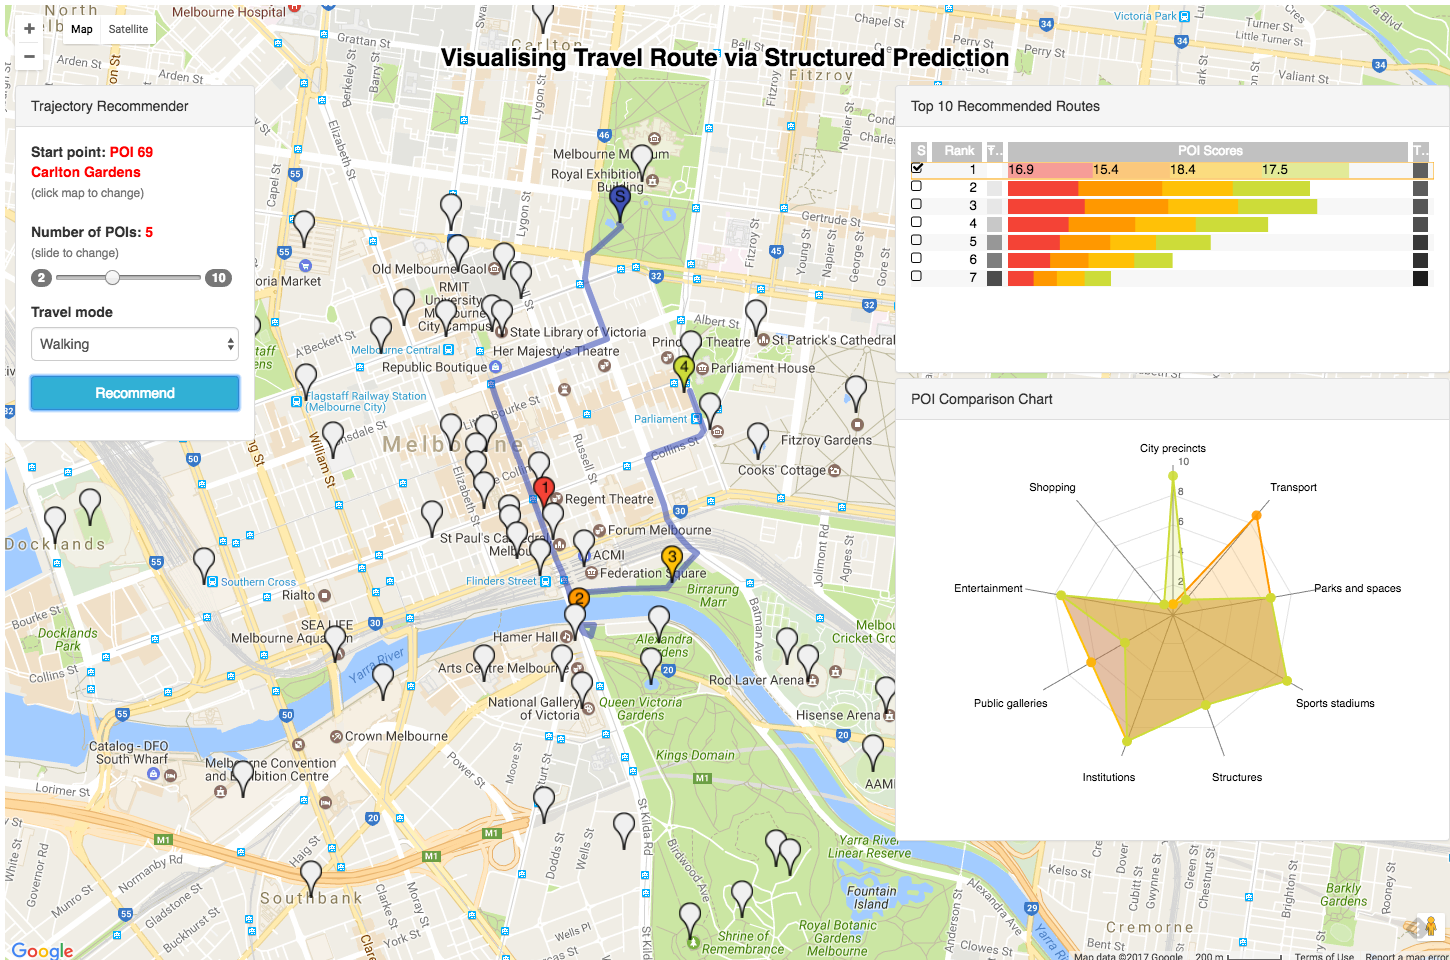
\includegraphics[width=\linewidth]{figure/sample_map2.png}
     \caption{Travel route visualisation system. Given a starting POI and a number of POI to be visited, the system recommends a set of routes from a history of previous tourists.}
   \label{fig:overview}
 \end{figure}
 
\section{Structured Prediction}
% don't need very details of the algorithm
% need problem definition
% copied from nips paper
Travel route recommendation problems involve a set of POIs in a city. 
Given a trajectory query $\mathbf{x} = (s, l)$, comprising a start POI $s$ and trip length $l$, the goal is to suggest one or more sequences of POIs that maximise some notion of utility.

We first cast travel recommendation as a structured prediction problem, which allows us to leverage the well-studied literature of structured SVMs (SSVM)~\cite{tsochantaridis2005large,joachims2009predicting}. 
There are two obstacles that prevent us from applying SSVM directly to the sequence recommendation problem; first, there would be multiple ground-truth routes among a set of POIs, second, a naive application of SSVM would generate a loop during prediction time. 
To incorporate multiple ground-truth routes in the learning phase, we take an idea from the ranking objective which prevents the ground-truth routes from competing with each others~\cite{rendle2009bpr}. 
To eliminate possible loops in prediction, we adopt the serial list Viterbi algorithm~\cite{seshadri1994list,nill1995list,nilsson2001sequentially}.
We finally trained our model on trajectory data extracted from Flickr photos taken in Melbourne~\cite{chen2016learning}.

From a visualisation perspective, an important advantage of the SSVM is the explicit representation of feature scores in its final decision process. Especially, in our case, we can disassemble the final score of a route into feature scores of each POI and each transition between two adjacency POIs. 
We use hand-crafted POI features such as the category, popularity, and average visit duration of previous tourists and also crafted transition features such as the distance and neighbourhood of two POIs to maximise the interpretability of the outcome.

\begin{figure}[t!]
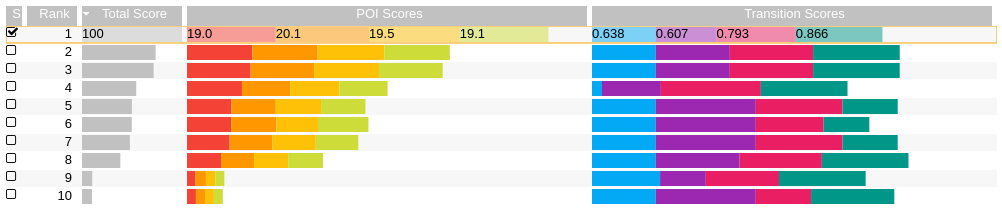
\includegraphics[width=0.9\linewidth]{figure/sample_stack.png}
\caption{Visualisation of POI scores for top ten recommended routes. Each bar from left to right represent a relative score of each POI along the route, and the total length of stacked bars represents the total score of the suggested route.}
\label{fig:stack}
\end{figure}
\section{Visualisation}
Our goal is to design an interactive visualisation system on top of the structured prediction framework.
Figure~\ref{fig:overview} shows the overview of a live demo system, which consists of five major components: a map to display suggested routes, an input box for user query (upper left), a stacked score of routes (upper right), a POI list (lower left), and a radar chart to compare features of multiple POIs (lower right). 
The role and the construction of the four major components, besides the main map, are as follows:

%\begin{itemize}
\textbf{Query input}: A query consists of a starting POI and a trip length. 
Users can choose the starting POI by clicking icons on the map and can adjust the slide to set the trip length. 
In addition, three different travelling modes (e.g. bicycling, walking, and driving) are supported, 
and we optimise the suggested routes for each mode.

\textbf{Route score visualisation}: 
The SSVM evaluates relevance scores of POIs and transitions in a candidate route to the given query and uses the sum of the relevance scores to determine the ranks of the routes.
To visualise the POI and transition scores, we adopt a stacked bar representation~~\cite{gratzl2013lineup}, designed to support the visualisation of multi-attribute ranking.
In Figure~\ref{fig:stack}, the system decompose the scores of top 10 recommended routes into POI and transition scores via the stacked bar representation, where the size of each bar is proportional to the relevance score of the corresponding POI and transition in the route.
Note that the POI and transition scores are scaled differently to support better visual discrimination\footnote{See Appendix for details at https://arxiv.org/abs/???.????}.
For each POI score, we also keep the same POI colour used to represent the POI on the map to support matching between a route on the map and bar plot seamlessly.

%Ranks of candidate routes are determined by their total scores from the SSVM. 
%The score of each route are decomposed into a set of scores for POIs and transitions along the route. 
%We adopt the LineUp framework~\cite{gratzl2013lineup} designed to support the visualisation of multi-attribute ranking via stacked representation. 
%To assist visualisation, both the POI and transition scores are properly scaled (see Appendix\footnote{https:arxiv.org/abs/???.????} for details).
%Figure~\ref{fig:stack} shows the stacked bars of the top 10 scored routes.
%Scores of different POI and transition are shown in different colours,
%and the proportion of each bar indicates the importance of the corresponding POI and transition in the route.
%At the left side, % of this representation,
%the user can select one or more suggested routes to get the numerical scores of POIs and transitions.
%All selected routes are drawn on the map, and the POIs in the most recent chosen route are shown with labelled icons.

\textbf{POI list}:
Users can select one or more suggested routes to get more detailed information. 
Specifically, information about the sequence of POIs in the selected route is provided, including POI names and their categories (e.g. Parks, Entertainment).
The POIs are ordered according to the suggested visiting order, with corresponding numerically labelled icons on the map.
The system also provides the estimated time and distance of the selected route at the top of this POI list.
When more than one route is selected, the system will display the POIs of the most recent chosen route.

\textbf{POI feature visualisation}: We further provide a radar chart to analyse the variation between POIs in a single route. 
For example, in Figure~\ref{fig:radar}, we compare two POIs, the \textit{Queen Victoria Market} and \textit{Melbourne Aquarium}, in terms of POI features and their importance in the suggested route. 
The radar chart shows the corresponding POI feature scores when a user selects a route.
In particular, the user can check/uncheck any POI in the selected route, and the feature scores of all checked POIs will be shown in the chart.
%\end{itemize}

\begin{figure}[t!]
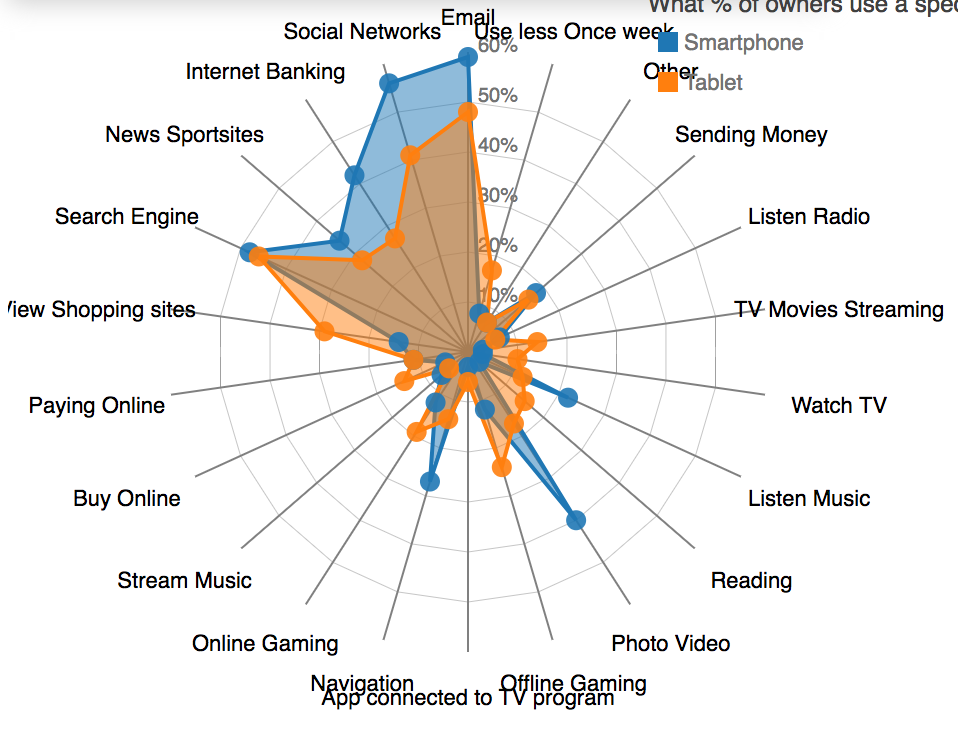
\includegraphics[width=0.6\linewidth]{figure/sample_radar.png} \vspace{-10pt}
    \caption{POI feature comparison between \textit{Melbourne Aquarium} and \textit{Queen Victoria Market}: the former scores higher on \textit{Popularity} and \textit{Visits difference} features whereas the latter scores higher on \textit{Visits} and \textit{Popularity difference} features.}
\label{fig:radar} \vspace{-1em}
\end{figure}

\section{Conclusion}
%summary
In this demonstration, we showcase an interactive route analyser which helps the interaction between users and route recommendation systems. 
The system benefits from the explicit feature construction of the structured prediction model and visualises recommended routes along with relevant information on both route and POI level.
As future work, it is of interest to incorporate %in the structured prediction model 
the amount of time tourists spent at each POI, 
and recommend the visit duration at POIs with proper visualisation as well.




\bibliographystyle{ACM-Reference-Format}
\bibliography{sigproc} 

\clearpage
\appendix
\onecolumn

\section{Description of the demonstrated system}
\label{sec:desc-sup}
% description of the demo system
The demonstrated system comprises two components, i.e. the server side and client side.
At the server side, a set of travel routes are generated from a trained structured SVMs as well as 
a query sent by the client. 
The generated routes are then sent to the client, which runs in a web browser, to visualise.
The server side was written in the Python programming language using \textit{pystruct}~\cite{JMLR:v15:mueller14a},
a Python library for structured learning and prediction,
as well as other essential Python libraries (with details below).
The client side was written in HTML, JavaScript and CSS.


% required setup
% website for users
\subsection{System setup}
\label{ssec:setup}
We created a website for users to try this system, it can be accessed at \url{http://115.146.87.43:8080/}.
As the source code of this system is hosted in a public GitHub repository, 
anyone interested in it can also run the system locally, by following the steps below:
\begin{enumerate}
\item Download the source code of the system from \url{https://github.com/cdawei/path_vis} 
% DW: move this to https://github.com/computationalmedia if it gets accepted?
\item Install the Python runtime and required libraries: 
      \begin{itemize}
      \item \textit{Python} version 3.5.3
      \item \textit{numpy} version 1.12.1 or newer
      \item \textit{scipy} version 0.19.0 or newer
      \item \textit{pandas} version 0.19.2
      \item \textit{scikit-learn} version 0.18.1 or newer
      \item \textit{joblib} version 0.11 or newer
      \item \textit{pystruct} version 0.2.4 or newer
      \end{itemize}
\item Go to the directory with system source code and launch the server slide: \texttt{python server.py}
\item Access \url{http://localhost:8080} using a web browser to use the visualisation system.
\end{enumerate}


%information about the presenters, including the relationship to the project
\subsection{Presenter}
\label{ssec:presenter}
The demonstrated system will be presented by Dawei Chen, a second year PhD student at the Australian National University.
The presenter is one of the member in a group that working on this project.


\end{document}
